\documentclass[a4paper,12pt]{article} 

%%% Работа с русским языком
\usepackage{cmap}					% поиск в PDF
\usepackage{mathtext} 				% русские буквы в фомулах
\usepackage[T2A]{fontenc}			% кодировка
\usepackage[utf8]{inputenc}			% кодировка исходного текста
\usepackage[english,russian]{babel}	% локализация и переносы

%%% Дополнительная работа с математикой
\usepackage{amsmath,amsfonts,amssymb,amsthm,mathtools, gensymb} % AMS
\usepackage{icomma} % "Умная" запятая: $0,2$ --- число, $0, 2$ --- перечисление

%%Таблица
\usepackage[table,xcdraw]{xcolor}
\usepackage{caption}
\usepackage{floatrow}
\floatsetup[table]{capposition=top}
\floatsetup[wrapfigure]{capposition=bottom}

%Отступы и поля 
\textwidth=18cm
\oddsidemargin=-1cm
\topmargin=-2cm
\textheight=25cm


%% Номера формул
\mathtoolsset{showonlyrefs=true} % Показывать номера только у тех формул, на которые есть \eqref{} в тексте.

%% Шрифты
\usepackage{euscript}	 % Шрифт Евклид
\usepackage{mathrsfs} % Красивый матшрифт

%% Свои команды
\DeclareMathOperator{\sgn}{\mathop{sgn}}

%% Перенос знаков в формулах (по Львовскому)
\newcommand*{\hm}[1]{#1\nobreak\discretionary{}
{\hbox{$\mathsurround=0pt #1$}}{}}

%% Стиль страницы
\usepackage{fancyhdr}

%% Для рисунков
\usepackage{graphicx}
\usepackage[export]{adjustbox}
\usepackage{float}
\usepackage{ragged2e}
\usepackage{wrapfig}

\pagestyle{fancy}
\begin{document}
\begin{titlepage}
\begin{center}
%\vspace*{1cm}
\large{\small ФЕДЕРАЛЬНОЕ ГОСУДАРСТВЕННОЕ АВТОНОМНОЕ ОБРАЗОВАТЕЛЬНОЕ\\ УЧРЕЖДЕНИЕ ВЫСШЕГО ОБРАЗОВАНИЯ \\ МОСКОВСКИЙ ФИЗИКО-ТЕХНИЧЕСКИЙ ИНСТИТУТ\\ (НАЦИОНАЛЬНЫЙ ИССЛЕДОВАТЕЛЬСКИЙ УНИВЕРСИТЕТ)\\ ФАКУЛЬТЕТ АЭРОКОСМИЧЕСКИХ ТЕХНОЛОГИЙ}
\vfill
\line(1,0){490}\\[1mm]
\huge{Лабораторная работа 3.3.2}\\
\huge\textbf{Исследование вольт-амперной характеристики ваккумного диода}\\
\line(1,0){490}\\[1mm]
\vfill
\begin{flushright}
\normalsize{Рогозин Владимир}\\
\normalsize{\textbf{Группа Б03-106}}\\
\end{flushright}
\end{center}
\end{titlepage}
\fancyhead[L] {Работа 3.3.2}


\textbf{Цель работы}: Определение удельного заряда электрона на основе закона
«трёх вторых» для вакуумного диода.


\textbf{Оборудование}: Вакуумная лампа с цилиндрическим анодом; амперметр; многопредельные микроамперметр и вольтметр постоянного тока; стабилизированные источники постоянного тока и постоянного напряжения.


\textbf{Теоретические сведения}: 
\begin{wrapfigure}[15]{l}{0.3\textwidth}\label{fig: diod}
    \begin{center}
    \vspace{-20pt}
        \includegraphics[width = 0.5\textwidth]{Diod.png}
    \end{center}
    \caption{Расположение электродов в диоде}
\end{wrapfigure}
\quad В работе исследуется зависимость величины тока, проходящего через вакуумный диод, от напряжения на нём.  Наибольший интерес представляет та область значений положительного напряжения на диоде, для которой пространственный заряд (электронное облако) в лампе существенно влияет на распределение электрического поля между катодом и анодом. Электрическое поле этого заряда «экранирует» поле вблизи катода, из-за чего лишь незначительная часть электронов, способных преодолеть энергетический барьер («работу выхода») и высвобождаемых из катода, создаёт ток через диод.

Выведем зависимость величины анодного тока от напряжения. Вакуумный диод имеет цилиндрическую форму, следовательно задача обладает цилиндрической симметрией,запишем теорему Гаусса в дифференциальной форме:

\begin{equation}\label{eq: diff Gauss Th}
    \frac{d}{dr}(r\frac{d\varphi}{dr}) = -\frac{r\rho}{\varepsilon_0}
\end{equation}
где $\rho$(r) -- объёмная плотность заряда, зависящая от расстояния до оси, граничные условия возьмём в виде 
\begin{equation}\label{eq: granich uslovia}
    \varphi (r_K) = 0,\quad  \varphi (r_A) = U
\end{equation}

В стационарном случае полный ток, пересекающий
цилиндрическую поверхность радиуса $r_K < r < r_A$ постоянен, следовательно
\begin{equation}\label{eq: I = const}
    I = -2\pi r\rho v l = const
\end{equation}
где $v$ -- скорость электронов, набираемая на пройденной ими разности потенциалов (начальной скоростью вылета электронов из катода пренебрегаем(предполагаем $eU\ll m{v_0}^2 / 2$), однако при малых напряжениях $U$ вклад начальной скорости может оказаться существенным, и  «закон 3/2» не будет выполняться):
\begin{equation}\label{eq: velocity via potential}
    \frac{mv^2}{2} = \varphi (r) - \varphi (r_K) =  \varphi (r)
\end{equation}

С помощью уравнений \eqref{eq: I = const}, \eqref{eq: velocity via potential} получаем уравнение:
\begin{equation}\label{eq: diff Gauss Th without velocity and density}
    \frac{d}{dr}(r\frac{d\varphi}{dr}) = \frac{I}{2\pi \varepsilon_0} \cdot\sqrt{\frac{m}{2e\varphi}}
\end{equation}

Также необходимо наложить ещё одно граничное условие, кототрое следует из условия $j_{max} \gg j$, то есть в предположении, что плотность тока в диоде значительно меньше максимального тока электронов, который может обеспечить катод. Тогда в предельном случае сколь угодно малые, отличные от нуля значения $E(r_A)$ приведут к неограниченному увеличению плотности тока $j$. это означает, что объёмный заряд вблизи катода полностью экранирует внешнее поле.
\[\left.\frac{d\varphi}{dr}\right|_{r = r_K}^{} = 0\]

Заметим, что если функция $\varphi_0(r)$ есть решение уравнения \eqref{eq: diff Gauss Th without velocity and density} при некотром $U_0$, которому сответствует сила тока $I_0$, введём функцию 
\[\varphi (r) = k\varphi_0 (r), \quad I = k^{3/2}\cdot I_0 \]
то уравнение \eqref{eq: diff Gauss Th without velocity and density} не изменит своего вида, отсюда находим, что 
\[\frac{U}{U_0} = k, \quad \frac{I}{I_0} = k^{3 / 2}, \quad I = I_0 \frac{U^{3/2}}{U_0^{3/2}}\]
легко установить, что $I \sim U^{3/2}$. Применимость данного закона ограничивается только двумя сделанными предположениями: 1) малость начальных скоростей электронов и 2) равенство нулю электричесокго поля на поверхности катода.

В пределе $r_K \rightarrow 0$ существует аналитическое решение уравнения \eqref{eq: diff Gauss Th without velocity and density} в виде $\varphi (r) = U\cdot {(r/r_A)}^{\beta}$. Подставив эту функцию в выражение \eqref{eq: diff Gauss Th without velocity and density}, найдём, что $\beta = 3/2$. Отсюда получаем зависимость силы анодного тока от напряжения:\
\begin{equation}\label{eq: I(U)}
    I = \beta \frac{4}{9}\varepsilon_0\frac{2\pi l}{r_A}\sqrt{\frac{2e}{m}}\cdot U^{3/2}
 \end{equation}
где $\beta$ -- коэффициент, зависящий от отношения $r_А$/$r_К$ ($\beta \rightarrow 1$ при $r_А$/$r_К \rightarrow 0$).

\textbf{Экспериментальная установка}: 
\begin{figure}[H]\label{fig: ustanovka}
    \centering
    \includegraphics{ustanovka.png}
    \caption{Схема экспериментальной установки}
\end{figure}

Исследования проводятся на диоде с косвенным накалом (ток пропускается через расположенную вблизи катода нить накала). Отметим, что длина $l$ меньше полной длины анода примерно в два раза. Благодаря этому рабочая часть катода достаточно удалена от его торцов, и следовательно, электрическое поле в активной части диода с хорошей точностью можно считать радиальным.

Схема экспериментальной установки изображена на рис. 2. Для питания цепи накала и анода используются два регулируемых источника напряжения. Ток накала $I_н$ измеряется амперметром. Анодное напряжение $U$ измеряется вольтметром, анодный ток $I$ — миллиамперметром.
\newpage

\textbf{Обработка данных}: Некоторые параметры диода: $r_А = 9,5$ мм, $l = 9$ мм, 
$\beta^2 = 0,95$ Перед началом измерений следует дать прогреться лампе 5--10 минут. Будем исследовать зависимость анодного тока от напряжения при четырёх различных значениях тока накала: $I_{н1} = 1.3 А$, $I_{н2} = 1.4 А$, $I_{н3} = 1.5 А$, $I_{н4} = 1.6 А$. Ниже в таблицах представлены результаты измерений анодного тока и напряжения:

\begin{table}[H]\label{tab: I(U) 1 and 2}
    \centering
    \begin{tabular}{|cc|cc|cc|}
        \hline
        \multicolumn{2}{|c|}{{\color[HTML]{000000} $I_н$ = 1,3A}} &
          \multicolumn{2}{c|}{{\color[HTML]{000000} $I_н$ = 1,4A}} &
          \multicolumn{2}{c|}{{\color[HTML]{000000} }} \\ \cline{1-4}
        \multicolumn{2}{|c|}{{\color[HTML]{000000} $I$, мкА}} &
           \multicolumn{2}{c|}{{\color[HTML]{000000} $I$, мкА}} &
           \multicolumn{2}{c|}{{{\color[HTML]{000000} $U$, В}}} \\ \hline
        \multicolumn{1}{|c|}{{\color[HTML]{000000} 3,62}} &
          {\color[HTML]{000000} 250,75} &
          \multicolumn{1}{c|}{{\color[HTML]{000000} 6,74}} &
          {\color[HTML]{000000} 274,76} &
          \multicolumn{1}{c|}{{\color[HTML]{000000} 0,5}} &
          {\color[HTML]{000000} 7,0} \\ \hline
        \multicolumn{1}{|c|}{{\color[HTML]{000000} 12,87}} &
          {\color[HTML]{000000} 309,82} &
          \multicolumn{1}{c|}{{\color[HTML]{000000} 17,79}} &
          {\color[HTML]{000000} 335,49} &
          \multicolumn{1}{c|}{{\color[HTML]{000000} 1,0}} &
          {\color[HTML]{000000} 8,0} \\ \hline
        \multicolumn{1}{|c|}{{\color[HTML]{000000} 23,33}} &
          {\color[HTML]{000000} 371,59} &
          \multicolumn{1}{c|}{{\color[HTML]{000000} 30,46}} &
          {\color[HTML]{000000} 400,94} &
          \multicolumn{1}{c|}{{\color[HTML]{000000} 1,5}} &
          {\color[HTML]{000000} 9,0} \\ \hline
        \multicolumn{1}{|c|}{{\color[HTML]{000000} 36,40}} &
          {\color[HTML]{000000} 443,68} &
          \multicolumn{1}{c|}{{\color[HTML]{000000} 45,71}} &
          {\color[HTML]{000000} 468,71} &
          \multicolumn{1}{c|}{{\color[HTML]{000000} 2,0}} &
          {\color[HTML]{000000} 10,0} \\ \hline
        \multicolumn{1}{|c|}{{\color[HTML]{000000} 50,95}} &
          {\color[HTML]{000000} 862,60} &
          \multicolumn{1}{c|}{{\color[HTML]{000000} 62,13}} &
          {\color[HTML]{000000} 909,50} &
          \multicolumn{1}{c|}{{\color[HTML]{000000} 2,5}} &
          {\color[HTML]{000000} 15,0} \\ \hline
        \multicolumn{1}{|c|}{{\color[HTML]{000000} 69,68}} &
          {\color[HTML]{000000} 1353,7} &
          \multicolumn{1}{c|}{{\color[HTML]{000000} 81,27}} &
          {\color[HTML]{000000} 1413,6} &
          \multicolumn{1}{c|}{{\color[HTML]{000000} 3,0}} &
          {\color[HTML]{000000} 20,0} \\ \hline
        \multicolumn{1}{|c|}{{\color[HTML]{000000} 87.44}} &
          {\color[HTML]{000000} 1929,0} &
          \multicolumn{1}{c|}{{\color[HTML]{000000} 101,54}} &
          {\color[HTML]{000000} 2005,9} &
          \multicolumn{1}{c|}{{\color[HTML]{000000} 3,5}} &
          {\color[HTML]{000000} 25,0} \\ \hline
        \multicolumn{1}{|c|}{{\color[HTML]{000000} 108,49}} &
          {\color[HTML]{000000} 2576,0} &
          \multicolumn{1}{c|}{{\color[HTML]{000000} 121,99}} &
          {\color[HTML]{000000} 2652,9} &
          \multicolumn{1}{c|}{{\color[HTML]{000000} 4,0}} &
          {\color[HTML]{000000} 30,0} \\ \hline
        \multicolumn{1}{|c|}{{\color[HTML]{000000} 129,60}} &
          {\color[HTML]{000000} 3264,6} &
          \multicolumn{1}{c|}{{\color[HTML]{000000} 146,11}} &
          {\color[HTML]{000000} 3360,4} &
          \multicolumn{1}{c|}{{\color[HTML]{000000} 4,5}} &
          {\color[HTML]{000000} 35,0} \\ \hline
        \multicolumn{1}{|c|}{{\color[HTML]{000000} 150,02}} &
          {\color[HTML]{000000} 4014,0} &
          \multicolumn{1}{c|}{{\color[HTML]{000000} 168,15}} &
          {\color[HTML]{000000} 4114,4} &
          \multicolumn{1}{c|}{{\color[HTML]{000000} 5,0}} &
          {\color[HTML]{000000} 40,0} \\ \hline
        \multicolumn{1}{|c|}{{\color[HTML]{000000} 173,79}} &
          {\color[HTML]{000000} 4816,1} &
          \multicolumn{1}{c|}{{\color[HTML]{000000} 192,32}} &
          {\color[HTML]{000000} 4926,8} &
          \multicolumn{1}{c|}{{\color[HTML]{000000} 5,5}} &
          {\color[HTML]{000000} 45,0} \\ \hline
        \multicolumn{1}{|c|}{{\color[HTML]{000000} 197,40}} &
          {\color[HTML]{000000} 5754,4} &
          \multicolumn{1}{c|}{{\color[HTML]{000000} 219,82}} &
          {\color[HTML]{000000} 5871,0} &
          \multicolumn{1}{c|}{{\color[HTML]{000000} 6,0}} &
          {\color[HTML]{000000} 50,0} \\ \hline
    \end{tabular}
    \caption{}
\end{table}

\begin{table}[H]\label{tab: I(U) 3 and 4}
    \centering
    \begin{tabular}{|cc|cc|cc|}
        \hline
        \multicolumn{2}{|c|}{{\color[HTML]{000000} $I_н$ = 1,5A}} &
          \multicolumn{2}{c|}{{\color[HTML]{000000} $I_н$ = 1,6A}} &
          \multicolumn{2}{c|}{{\color[HTML]{000000} }} \\ \cline{1-4}
        \multicolumn{2}{|c|}{{\color[HTML]{000000} $I$, мкА}} &
          \multicolumn{2}{c|}{{\color[HTML]{000000} $I$, мкА}} &
          \multicolumn{2}{c|}{{{\color[HTML]{000000} $U$, В}}} \\ \hline
        \multicolumn{1}{|c|}{{\color[HTML]{000000} 12,54}} &
          {\color[HTML]{000000} 304,02} &
          \multicolumn{1}{c|}{{\color[HTML]{000000} 21,12}} &
          {\color[HTML]{000000} 332,77} &
          \multicolumn{1}{c|}{{\color[HTML]{000000} 0,5}} &
          {\color[HTML]{000000} 7,0} \\ \hline
        \multicolumn{1}{|c|}{{\color[HTML]{000000} 24,04}} &
          {\color[HTML]{000000} 364,0} &
          \multicolumn{1}{c|}{{\color[HTML]{000000} 35,89}} &
          {\color[HTML]{000000} 398,95} &
          \multicolumn{1}{c|}{{\color[HTML]{000000} 1,0}} &
          {\color[HTML]{000000} 8,0} \\ \hline
        \multicolumn{1}{|c|}{{\color[HTML]{000000} 40,02}} &
          {\color[HTML]{000000} 460,0} &
          \multicolumn{1}{c|}{{\color[HTML]{000000} 53,77}} &
          {\color[HTML]{000000} 467,95} &
          \multicolumn{1}{c|}{{\color[HTML]{000000} 1,5}} &
          {\color[HTML]{000000} 9,0} \\ \hline
        \multicolumn{1}{|c|}{{\color[HTML]{000000} 36,40}} &
          {\color[HTML]{000000} 535,59} &
          \multicolumn{1}{c|}{{\color[HTML]{000000} 71,57}} &
          {\color[HTML]{000000} 575,40} &
          \multicolumn{1}{c|}{{\color[HTML]{000000} 2,0}} &
          {\color[HTML]{000000} 10,0} \\ \hline
        \multicolumn{1}{|c|}{{\color[HTML]{000000} 56,47}} &
          {\color[HTML]{000000} 951,20} &
          \multicolumn{1}{c|}{{\color[HTML]{000000} 93,52}} &
          {\color[HTML]{000000} 1004,3} &
          \multicolumn{1}{c|}{{\color[HTML]{000000} 2,5}} &
          {\color[HTML]{000000} 15,0} \\ \hline
        \multicolumn{1}{|c|}{{\color[HTML]{000000} 76,02}} &
          {\color[HTML]{000000} 1473,3} &
          \multicolumn{1}{c|}{{\color[HTML]{000000} 112,42}} &
          {\color[HTML]{000000} 1541,1} &
          \multicolumn{1}{c|}{{\color[HTML]{000000} 3,0}} &
          {\color[HTML]{000000} 20,0} \\ \hline
        \multicolumn{1}{|c|}{{\color[HTML]{000000} 96,01}} &
          {\color[HTML]{000000} 2073,3} &
          \multicolumn{1}{c|}{{\color[HTML]{000000} 136,48}} &
          {\color[HTML]{000000} 2148,2} &
          \multicolumn{1}{c|}{{\color[HTML]{000000} 3,5}} &
          {\color[HTML]{000000} 25,0} \\ \hline
        \multicolumn{1}{|c|}{{\color[HTML]{000000} 117,30}} &
          {\color[HTML]{000000} 2729,6} &
          \multicolumn{1}{c|}{{\color[HTML]{000000} 162,59}} &
          {\color[HTML]{000000} 2822,4} &
          \multicolumn{1}{c|}{{\color[HTML]{000000} 4,0}} &
          {\color[HTML]{000000} 30,0} \\ \hline
        \multicolumn{1}{|c|}{{\color[HTML]{000000} 163,58}} &
          {\color[HTML]{000000} 3448,4} &
          \multicolumn{1}{c|}{{\color[HTML]{000000} 188,02}} &
          {\color[HTML]{000000} 3546,7} &
          \multicolumn{1}{c|}{{\color[HTML]{000000} 4,5}} &
          {\color[HTML]{000000} 35,0} \\ \hline
        \multicolumn{1}{|c|}{{\color[HTML]{000000} 188,60}} &
          {\color[HTML]{000000} 4219,4} &
          \multicolumn{1}{c|}{{\color[HTML]{000000} 211,7}} &
          {\color[HTML]{000000} 4321,3} &
          \multicolumn{1}{c|}{{\color[HTML]{000000} 5,0}} &
          {\color[HTML]{000000} 40,0} \\ \hline
        \multicolumn{1}{|c|}{{\color[HTML]{000000} 214,25}} &
          {\color[HTML]{000000} 5033,2} &
          \multicolumn{1}{c|}{{\color[HTML]{000000} 239,24}} &
          {\color[HTML]{000000} 5231,0} &
          \multicolumn{1}{c|}{{\color[HTML]{000000} 5,5}} &
          {\color[HTML]{000000} 45,0} \\ \hline
        \multicolumn{1}{|c|}{{\color[HTML]{000000} 239,59}} &
          {\color[HTML]{000000} 5990,0} &
          \multicolumn{1}{c|}{{\color[HTML]{000000} 267,88}} &
          {\color[HTML]{000000} 6117,0} &
          \multicolumn{1}{c|}{{\color[HTML]{000000} 6,0}} &
          {\color[HTML]{000000} 50,0} \\ \hline
    \end{tabular}
    \caption{}
\end{table}

Далее, построим графики зависимостей $ln(I)(ln(U))$ для каждого из значений тока накала.

\begin{figure}[H]\label{fig: ln(I)(ln(U)) 1.3}
    \centering
    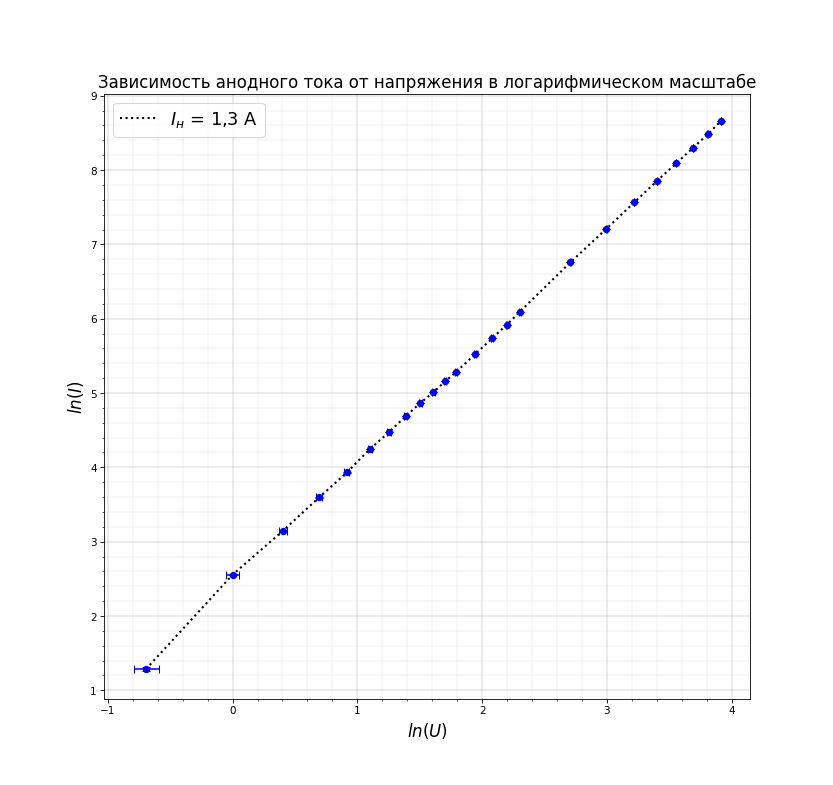
\includegraphics[width = \textwidth]{ln(I)(ln(U))_13.png}
\end{figure}

Из графика найдем коэффициент наклона прямой, сравним его с теоретическим значением $k = 3/2$:
\[k_{1,3} = (1,578 \pm 0,005), \quad \varepsilon_k = 0,32\% \]
значение отличается от теоретически предсказанного на $\approx 5\%$. Видно, что практически во всем диапазоне напряжений зависимость получается линейной с хорошей точностью. Все погрешности точек на графике здесь и далее расчитаны по формуле
\[a = f(x_1, x_2, ... , x_n)\]
\[\sigma_a = \sum {\frac{\partial f}{\partial x_i}}^2\cdot {\sigma_{x_i}}^2\]
\begin{figure}[H]\label{fig: ln(I)(ln(U)) 1.4}
    \centering
    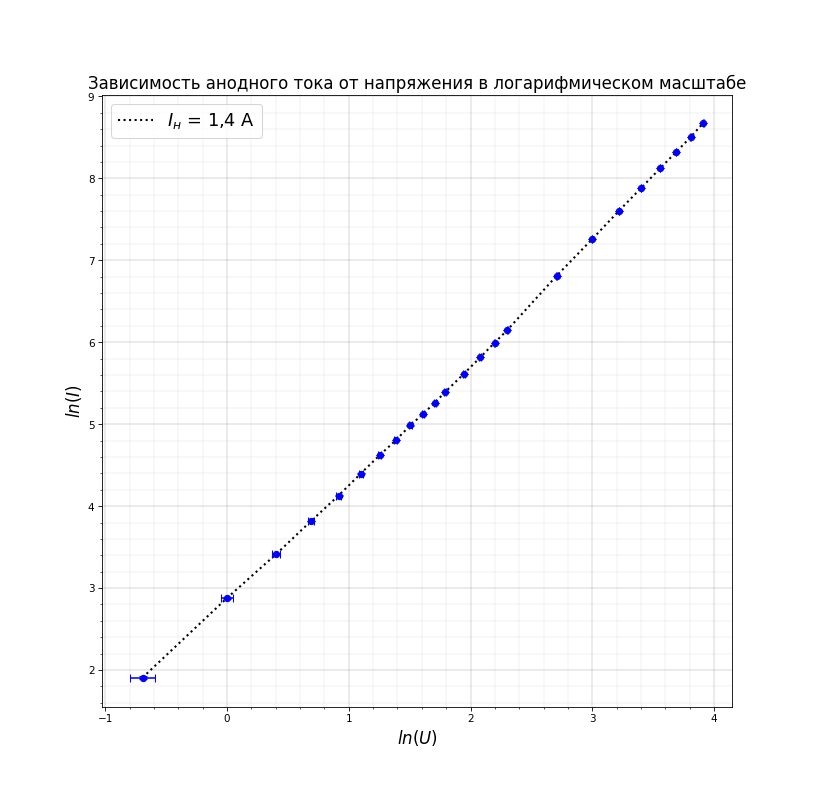
\includegraphics[width = \textwidth]{ln(I)(ln(U))_14.png}
\end{figure}
\[k_{1,4} = (1,487 \pm 0,010), \quad \varepsilon_k = 0,67\% \]
значение отличается от 3/2 меньше чем на $ 1\%$. При токе накала $I_н = 1,4 \text{ }A$ 
зависимость все ещё линейна с хорошей точностью.
\begin{figure}[H]\label{fig: ln(I)(ln(U)) 1.5}
    \centering
    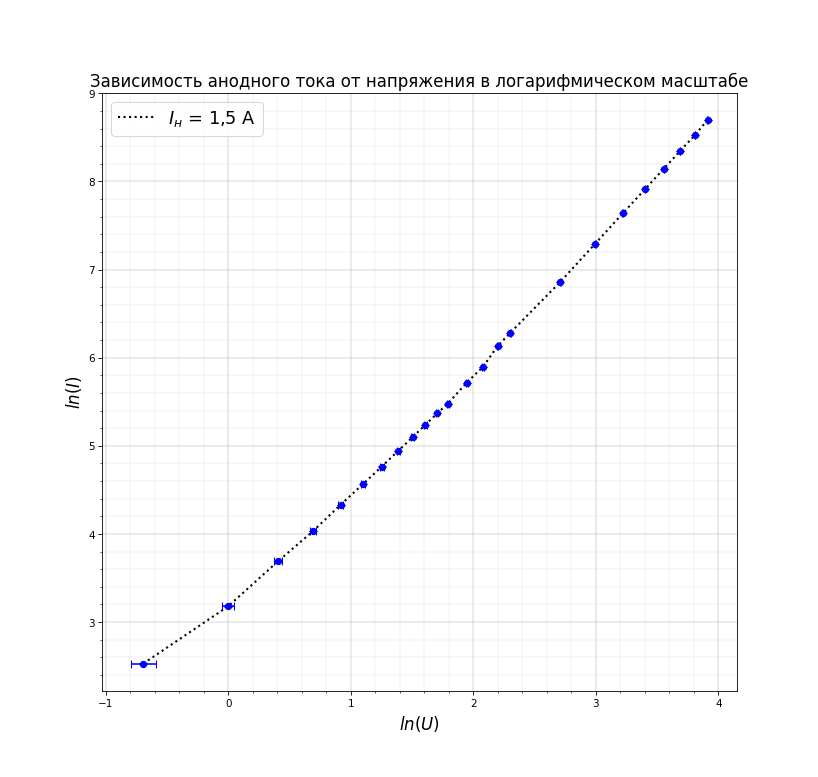
\includegraphics[width = \textwidth]{ln(I)(ln(U))_15.png}
\end{figure}
При токе накала $I_н = 1,5 \text{ }A$ точки хуже ложатся на прямую, в основном из-за первых трёх, завышенные значения которых могут быть связаны с тем, что при малых напряжениях и вклад в начальную скорость электронов может сносить тепловое движение, которое тем существеннее, чем больше ток накала, поэтому такого отклонения не наблюдалось при меньших токах. Посчитаем коэффициент $k$ без учёта первых трёх точек:
\[k_{1,5} = (1,465 \pm 0,009), \quad \varepsilon_k = 0,61\% \]
значение отличается от предполагаемого на $\approx 2,5 \%$. За исключением первых трёх точек зависимость линейна.
\begin{figure}[H]\label{fig: ln(I)(ln(U)) 1.6}
    \centering
    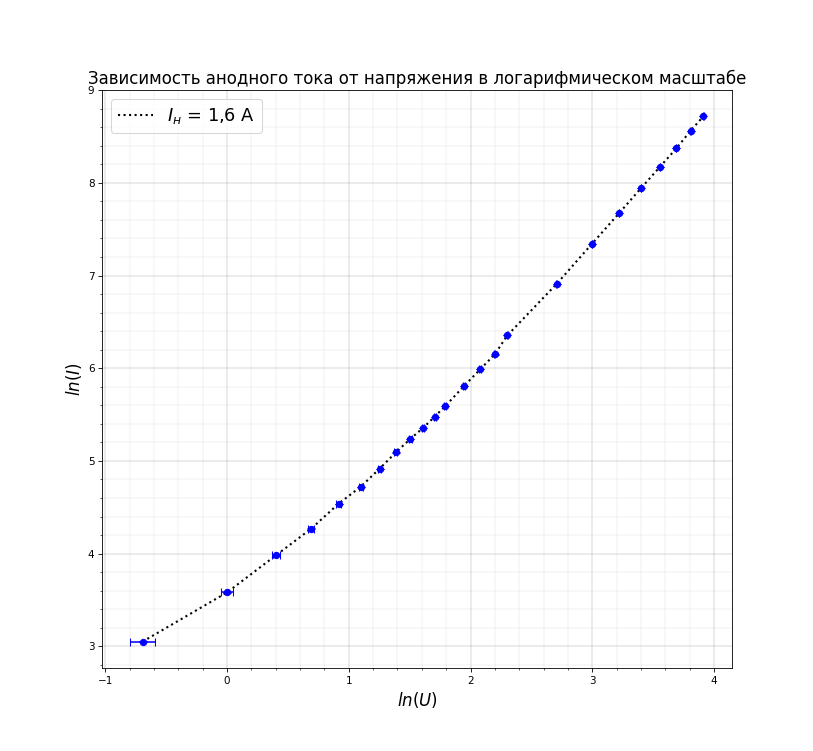
\includegraphics[width = \textwidth]{ln(I)(ln(U))_16.png}
\end{figure}
Опять заметим, что значения тока в первых трёх точках явно завышены(по сравнению с теорией), как и в предыдущем случае, это может быть вызвано влиянием тепловых скоростей. Расчитаем угол наклона исключая первые три точки из рассмотрения:
\[k_{1,6} = (1,408 \pm 0,014), \quad \varepsilon_k = 0,99\% \]
значение отличается от предполагаемого на $\approx 6,5 \%$. Как и в предыдущем случае, за исключением первых трёх точек зависимость близка к линейной.

Теперь построим графики зависимости $I(U^{3/2})$, по углу наклона прямой найдём коэффициент пропорциональности, по формуле \eqref{eq: I(U)} рассчитаем удельный заряд $e$/$m$:
\[\frac{e}{m} = \frac{1}{\beta^2}\frac{81}{128}\frac{k^2\cdot {r_A}^2}{{\pi}^2{\varepsilon_0}^2 l^2}\]


\begin{figure}[H]\label{fig: I)(U^3/2) 1.3}
    \centering
    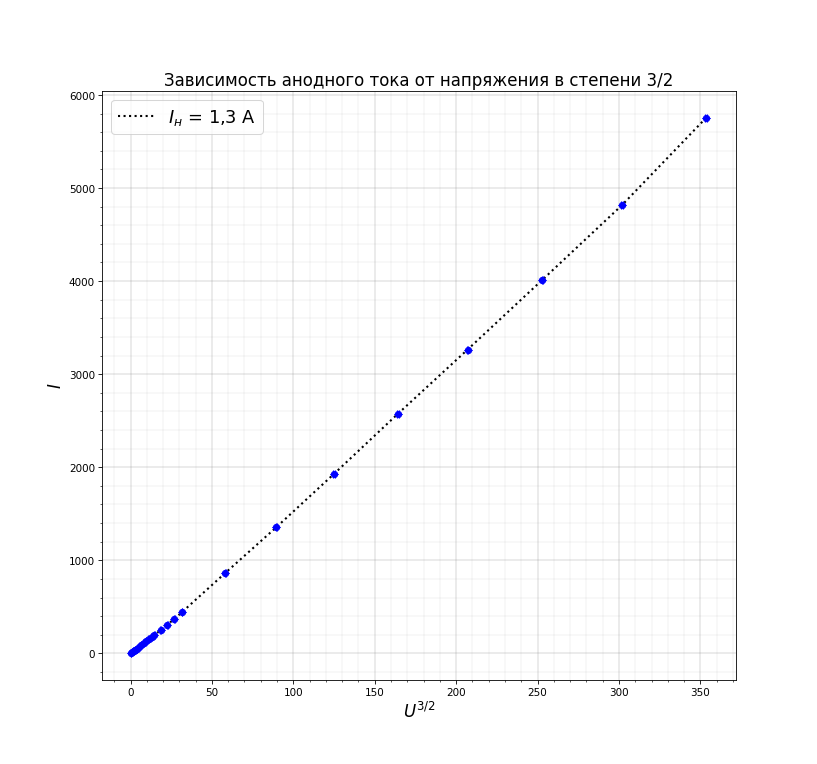
\includegraphics[width = \textwidth]{I(U pow (1,5))_13.png}
\end{figure}
\[k_{1,3} = (16,10 \pm 0,07), \quad \varepsilon_k = 0,43\% \]
\[\frac{e}{m} = (246,0 \pm 2,1) \cdot 10^{9} \text{ } Кл \cdot кг^{-1}, \quad \varepsilon = 2\varepsilon_k = 0,86\%\]
Табличное значение удельного заряда: $e / m = 176\cdot 10^{9} \text{ } Кл \cdot м^{-1}$.
Полученное значение отличается от табличного на $\approx 40\%$, что является плохим результатом. 

\begin{figure}[H]\label{fig: I)(U^3/2) 1.4}
    \centering
    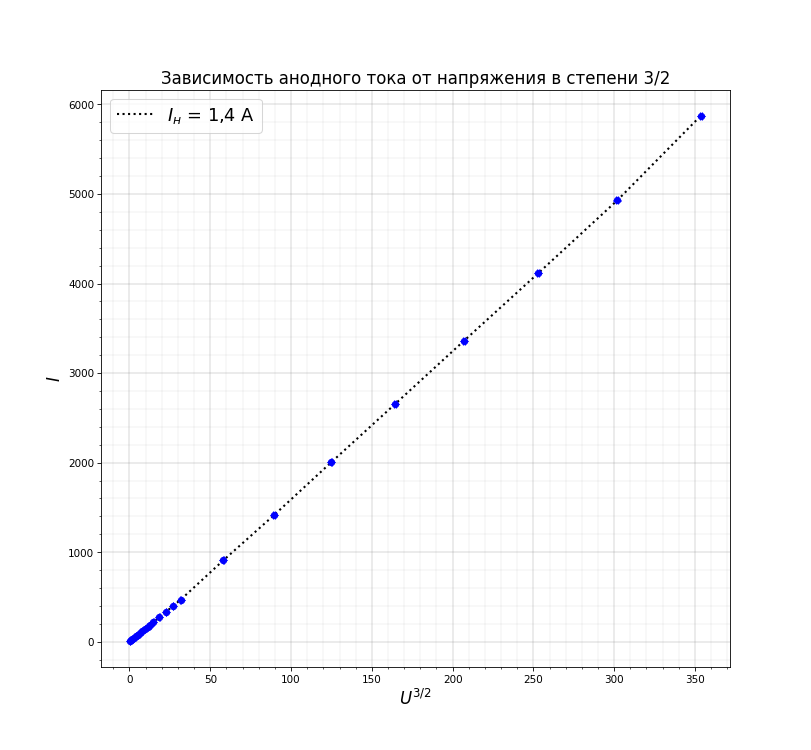
\includegraphics[width = \textwidth]{I(U pow (1,5))_14.png}
\end{figure}
\[k_{1,4} = (16,44 \pm 0,05), \quad \varepsilon_k = 0,30\% \]
\[\frac{e}{m} = (256,7 \pm 1,5) \cdot 10^{9} \text{ } Кл \cdot кг^{-1}, \quad \varepsilon = 2\varepsilon_k = 0,60\%\]
Результат отличается от табличного значения на $\approx 45\%$, что получается ещё хуже, чем в первом случае.

\begin{figure}[H]\label{fig: I)(U^3/2) 1.5}
    \centering
    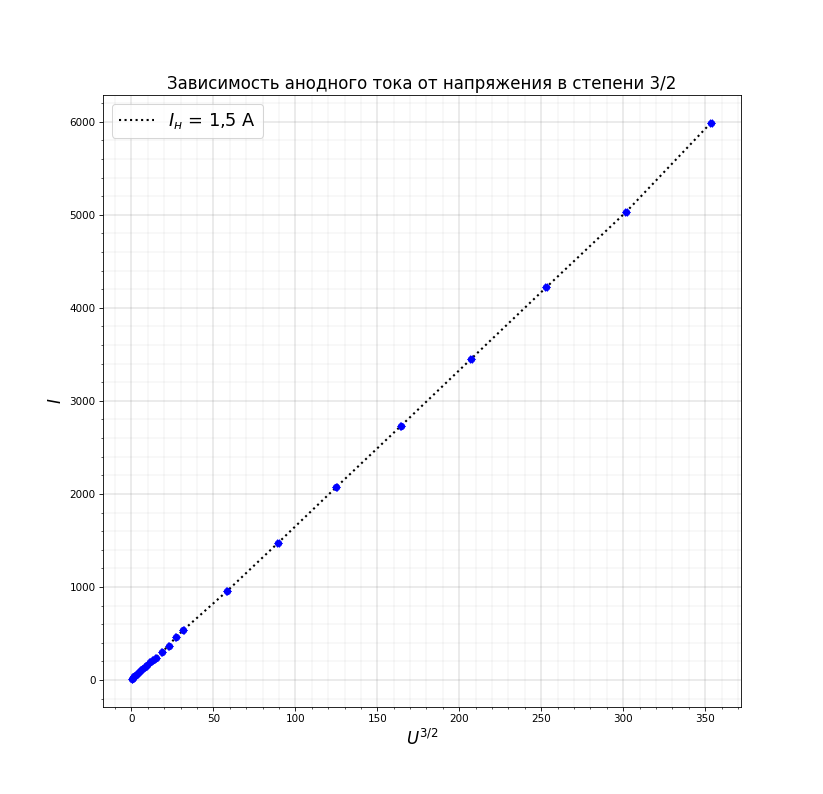
\includegraphics[width = \textwidth]{I(U pow (1,5))_15.png}
\end{figure}
\[k_{1,5} = (17,10 \pm 0,07), \quad \varepsilon_k = 0,55\% \]
\[\frac{e}{m} = (266,7 \pm 2,9) \cdot 10^{9} \text{ } Кл \cdot кг^{-1}, \quad \varepsilon = 2\varepsilon_k = 1,10\%\]
В этом случае первые три точки почти не вносят изменений в коэффициент наклона прямой и его погрешность, поэтому можно их не выкидывать. Полученный удельный заряд отличается от табличного на $\approx  51\%$, что может указывать на то, что чем выше ток накала, тем хуже выполняется "закон трёх-вторых".

\begin{figure}[H]\label{fig: I)(U^3/2) 1.6}
    \centering
    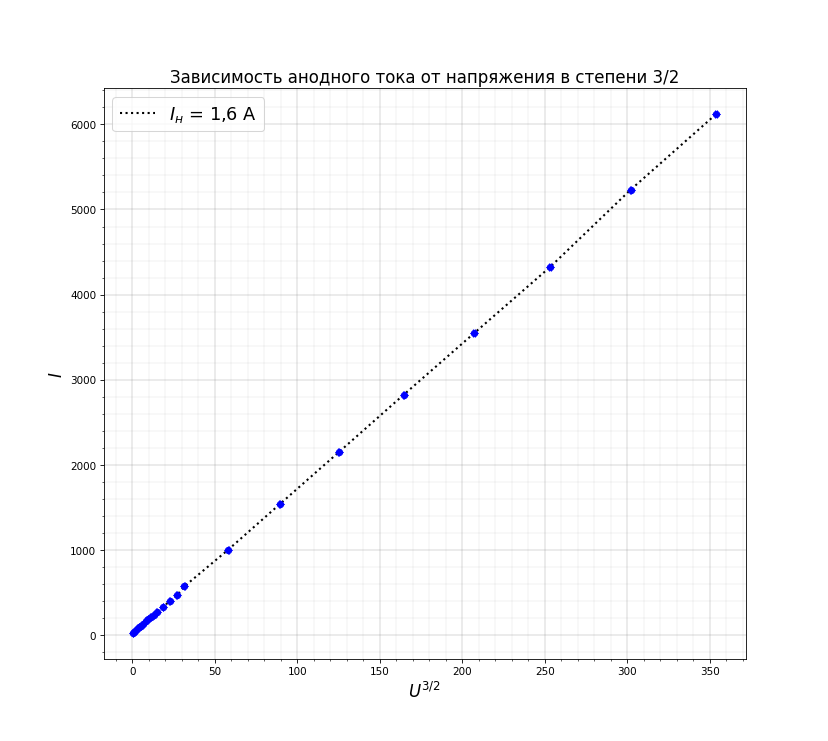
\includegraphics[width = \textwidth]{I(U pow (1,5))_16.png}
\end{figure}
\[k_{1,6} = (17,15 \pm 0,07), \quad \varepsilon_k = 0,54\% \]
\[\frac{e}{m} = (268,2 \pm 2,9) \cdot 10^{9} \text{ } Кл \cdot кг^{-1}, \quad \varepsilon = 2\varepsilon_k = 1,08\%\]
Аналогично предыдущему случаю, коэффициент наклона будем искать беря все точки. В последнем случае отличие значения от табличного составляет $\approx 52\%$, что ещё лучше подтверждает границы применимости "закона трёх-вторых".


\textbf{Вывод}: В данной работе исследовался "закон трёх-вторых" для вакуумного диода, с его помощью рассчитывался удельный заряд электрона. Количественный результат сильно не совпал с табличным значением (погрешность наилучшего значения $\approx 40\%$, наихудшего $\approx 52\%$). Однако, предположение о границах применимости данного закона подтвердилась экспериментом -- при больших значениях тока накала всё больше влияла тепловая скорость электронов, и значение удельного заряда электрона, полученное с помощью формулы, не учитывающей тепловое движение, всё больше отличалось от табличного. 

\end{document}
